
\setcounter{chapter}{2}
\chapter{System Design and Architecture}
\minitoc %insert la minitoc
\graphicspath{{Chapitre3/figures/}}

%\DoPToC
%==============================================================================
\pagestyle{fancy}
\fancyhf{}
\fancyhead[R]{\bfseries\rightmark}
\fancyfoot[R]{\thepage}
\renewcommand{\headrulewidth}{0.5pt}
\renewcommand{\footrulewidth}{0pt}
\renewcommand{\chaptermark}[1]{\markboth{{\chaptername~\thechapter. #1 }}{}}
\renewcommand{\sectionmark}[1]{\markright{\thechapter.\thesection~ #1}}

\begin{spacing}{1.2}

%==============================================================================
\section*{Introduction}
This chapter presents the system design and architecture of the LLM-powered best practices enforcement system. Building on the business understanding and requirements established in the previous chapter, this chapter details the technical design decisions, architectural patterns, and system components that enable real-time, intelligent feedback for YouTube framework development.

The design follows traditional software engineering principles while incorporating modern AI technologies. This chapter covers the overall system architecture, component design, data models, and integration patterns that form the foundation of the implemented solution.

\section{System Architecture Overview}

\subsection{High-Level Architecture}
The system architecture is designed to integrate seamlessly into the developer's existing workflow while providing intelligent, context-aware feedback. The architecture consists of two main components that work together to deliver real-time best practice enforcement:

\begin{itemize}
    \item \textbf{IDE}: The developer's workspace containing the YouTube IDE Extension, which works with the currently open file being analyzed and annotates results directly in the editor.
    \item \textbf{AI Agent Framework}: The processing layer containing the LLM Best Practices Agent, which serves as the core AI processing engine that uses internal LLMs to analyze code and suggest best practices.
\end{itemize}

\begin{figure}[H]
\centering
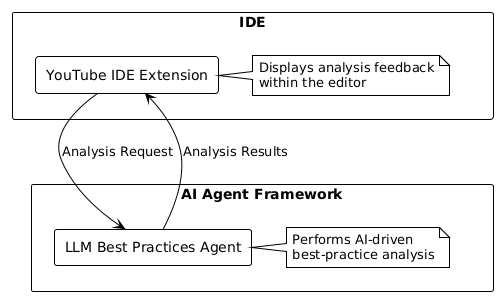
\includegraphics[scale=0.7]{images/high_level_system_architecture.png}
\caption{High-Level System Architecture}
\label{fig:system_architecture}
\end{figure}

\subsection{System Workflow}
The system operates through a streamlined workflow that begins when a developer triggers analysis via the YouTube IDE Extension. The complete interaction flow is depicted in Figure \ref{fig:sequence_diagram}.

\begin{figure}[H]
\centering
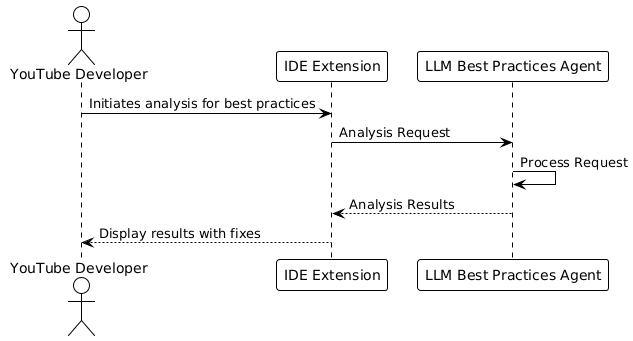
\includegraphics[scale=0.7]{images/sequence_diagram.png}
\caption{System Interaction Sequence Diagram}
\label{fig:sequence_diagram}
\end{figure}

The sequence unfolds through the following interactions and responsibilities:
\begin{enumerate}
    \item \textbf{Analysis initiation}: The YouTube developer triggers analysis of the currently open file.
    \item \textbf{Request submission}: The YouTube IDE Extension submits an analysis request to the agent, identifying the target file.
    \item \textbf{Processing}: The agent performs best-practices analysis and prepares the resulting findings.
    \item \textbf{Result delivery}: The agent returns a structured response to the YouTube IDE Extension.
    \item \textbf{Presentation}: The YouTube IDE Extension presents the best practices violations and suggested fixes within the editor.
\end{enumerate}

This workflow emphasizes decoupling the IDE from heavy AI computation, ensuring that the development environment remains responsive while delegating intensive analysis to the specialized agent framework.

\section{Components Design}

\subsection{LLM Best Practices Agent} 
The LLM Best Practices Agent serves as the core intelligence engine of the system, responsible for analyzing code, identifying violations of YouTube framework best practices, and providing actionable feedback to developers. This component represents the convergence of modern AI capabilities with domain-specific software engineering expertise.

\subsubsection{Agent Architecture Choice}
The agent is built using the Executable Agent architecture, provided by our internal AI platform. This architecture offers a structured approach to orchestrating AI-powered workflows, and was selected after careful evaluation of different agent paradigms, considering reliability, performance, and maintainability.

\paragraph{Executable Agent vs. ReAct Architecture}
To motivate the choice of Executable Agent architecture, we contrast it with the more widely known ReAct (Reasoning and Acting) pattern. In our system, the Executable Agent refers to a deterministic, tool-orchestrated workflow where control flow is defined in code rather than delegated to LLM reasoning. For readers outside Google, this is conceptually similar to what Microsoft publicly describes as sequential orchestration~\cite{microsoftAgentPatterns}, though our implementation is independent and internally developed.

\begin{itemize}
    \item \textbf{ReAct Agent}: Uses a reasoning loop where the LLM decides what action to take next, executes it, observes the result, and continues reasoning. This creates a dynamic, LLM-driven execution flow.
    \item \textbf{Executable Agent}: Follows a predefined, deterministic execution flow where the agent orchestrates a sequence of tool calls in a structured manner, with the LLM used primarily for processing within each tool rather than for orchestration decisions.
\end{itemize}


Figure~\ref{fig:agent_comparison} illustrates the fundamental difference in control flow between the two approaches.

\begin{figure}[H] 
	\centering 
	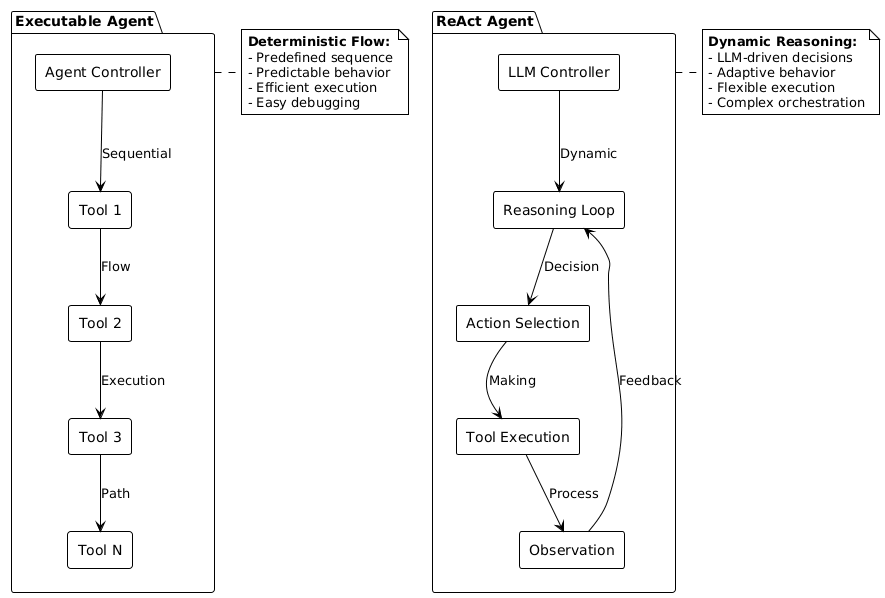
\includegraphics[scale=0.6]{images/agent_architecture_comparison.png} 
	\caption{Comparison of Executable Agent vs. ReAct Agent Architectures} 
	\label{fig:agent_comparison} 
\end{figure}

The Executable Agent architecture offers several key advantages for this use case:
\begin{itemize}
    \item \textbf{Deterministic Execution}: Predefined flow ensures predictable behavior and simplifies debugging.
    \item \textbf{Tool Orchestration}: Clean framework for coordinating multiple specialized tools.
    \item \textbf{Error Handling}: Built-in mechanisms for handling failures and graceful degradation.
    \item \textbf{Performance (Latency)}: Efficient execution with low response latency, since orchestration decisions are pre-programmed rather than deferred to open-ended LLM reasoning.
    \item \textbf{Cost Efficiency (Token Usage)}: Reduced token consumption by constraining LLM calls to focused, well-scoped processing steps rather than repeated reasoning loops.
    \item \textbf{Maintainability}: Clear separation of concerns between tools and responsibilities.
\end{itemize}



\subsubsection{Core Tools Architecture}
To achieve this structured workflow, the agent incorporates five specialized tools, each handling a specific step of the best practices analysis pipeline.
\paragraph{ReadFileFromWorkspace Tool}
This tool serves as the entry point for code analysis, responsible for retrieving the complete content of the file being analyzed. It handles file system access, ensuring that the agent has access to the full context of the code under examination. The tool is designed to handle multiple file formats and encodings that might arise in different development environments. Design contract: input = file path; output = full file content.

\paragraph{CodeAnalysisTool}
The core analysis engine that performs violation detection against YouTube framework best practices. This tool uses an internal Large Language Model to perform semantic code analysis, going beyond simple pattern matching to understand intent and context. It can identify violations related to:
\begin{itemize}
    \item Framework-specific patterns and anti-patterns
    \item Component structure and organization
    \item Code complexity and maintainability
    \item Import patterns and dependencies
    \item Naming conventions
\end{itemize}
Design contract: input = file content + convention set; output = list of base violations.

\paragraph{ViolationExplanationTool}
This tool leverages the internal Large Language Model to generate human-readable explanations for each identified violation, providing developers with clear understanding of why a particular code pattern violates best practices. The explanations are contextual and educational, helping developers not only fix the immediate issue but also understand the underlying principles. Design contract: input = base violation + surrounding code context + convention; output = natural-language explanation.

\paragraph{CodeFixTool}
This tool uses the same internal Large Language Model to propose actionable fix suggestions for identified violations. It goes beyond simply identifying problems to provide concrete solutions that developers can implement. Design contract: input = base violation + explanation + code context; output = suggested fix. The fixes are designed to be:
\begin{itemize}
    \item \textbf{Safe}: Only modify internal implementation without breaking public APIs
    \item \textbf{Self-contained}: Require no additional changes in other files
    \item \textbf{Contextual}: Take into account the specific code context and framework patterns
    \item \textbf{Educational}: Include comments explaining the reasoning behind the fix
\end{itemize}

\paragraph{Finish Tool}
The consolidation component that aggregates all analysis results into a structured output format. This tool ensures that the response is properly formatted and contains all necessary information for the YouTube IDE Extension to display results effectively. It enforces the response schema, deduplicates entries, and merges overlapping ranges when applicable, producing a coherent set of violations, explanations, and fixes.

\subsubsection{Processing Strategy}
The agent employs a balanced processing strategy that weighs performance against reliability. This strategy represents a key architectural decision made after evaluating different processing approaches for handling multiple violations within a single file.

\paragraph{Processing Strategy Options}
During the design phase, three main processing strategies were considered for handling multiple violations:

\begin{itemize}
    \item \textbf{Fully Sequential Processing}: Each violation is processed one at a time, with explanation generation and fix creation happening sequentially for each violation. This approach ensures maximum reliability and predictability but may result in longer processing times for files with many violations.
    
    \item \textbf{Fully Parallel Processing}: All violations are processed concurrently, with explanation generation and fix creation happening simultaneously for all violations. This approach maximizes performance but introduces complexity in managing concurrent operations and may face reliability challenges under high load conditions.
    
    \item \textbf{Hybrid Parallel Processing with Concurrency Limiting}: A balanced approach that processes violations in parallel but with controlled concurrency to maintain system stability. This strategy provides significant performance improvements over sequential processing while ensuring reliable operation even under various load conditions.
\end{itemize}

The hybrid parallel processing strategy with concurrency limiting was selected as it provides the optimal balance between performance and reliability for production use. The internal workflow is illustrated in the activity diagram below:


\begin{figure}[H]
	\centering
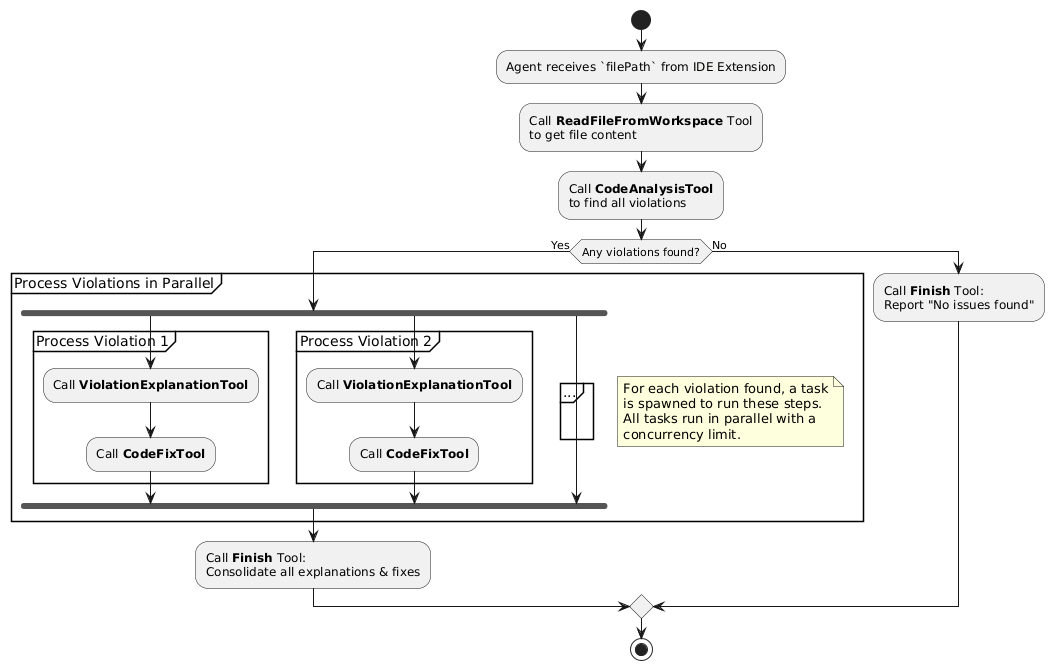
\includegraphics[scale=0.5]{images/activity_diagram.png}
\caption{Agent Processing Activity Diagram}
\label{fig:agent_activity}
\end{figure}

The workflow demonstrates the key architectural decisions made in the processing strategy:

\paragraph{Sequential Initial Processing}
The agent begins with sequential steps: file reading and violation detection. This ensures that the complete code context is available before any analysis begins, and all violations are identified before parallel processing starts.

\paragraph{Parallel Violation Processing}
When violations are found, the agent employs the hybrid parallel processing strategy with concurrency limiting. Each violation is processed independently, with explanation generation and fix creation happening concurrently across multiple violations while maintaining system stability. A default concurrency limit is applied, and excess tasks are queued to prevent resource saturation. LLM calls use bounded retries with exponential backoff; on persistent failure, partial results are returned. Failures are isolated per violation—an error in one task does not stop processing of other violations.

\paragraph{Result Consolidation}
The workflow concludes with result consolidation, ensuring that all parallel processing results are properly aggregated into a coherent response format for the YouTube IDE Extension.

\subsubsection{Integration with LLM Infrastructure}
The agent integrates with an internal AI platform that hosts multiple LLMs. We currently use the latest internal Gemini‑based model trained on Google's codebase. The architecture is model‑agnostic, enabling seamless adoption of newer Gemini‑based models as they are released without requiring changes in the orchestration logic. LLM usage is isolated behind stable interfaces so higher‑level logic remains unaffected. Three tools depend on the LLM: CodeAnalysisTool, ViolationExplanationTool, and CodeFixTool. Integration concerns include prompt construction, response parsing, error handling, and token‑usage tracking. Token usage monitoring is crucial for both cost management and latency optimization, enabling capacity planning and performance tuning. This design ensures long‑term maintainability and benefits from platform improvements without architectural change.

\subsection{YouTube IDE Extension}
The YouTube IDE Extension serves as the user-facing interface that seamlessly integrates the LLM Best Practices Agent into YouTube developers' daily workflow. Since YouTube developers are the primary target audience for this system, the YouTube IDE Extension was chosen as the natural entry point, leveraging their existing development environment and workflow patterns. This component is designed to provide intelligent, context-aware feedback while maintaining the responsiveness and familiarity that developers expect from their development environment. The feature becomes available when developers enable a user setting in the extension, and entry points only appear for files that belong to the internal YouTube framework for which we enforce best practices.

\subsubsection{Extension Architecture}
The YouTube IDE Extension is designed as a lightweight client that orchestrates the interaction between the developer and the AI analysis system. The architecture ensures that the extension remains responsive while delegating computationally intensive analysis to the specialized agent framework.

The extension handles user interface concerns, progress indication, and result presentation, while the heavy lifting of code analysis and AI processing is handled by the dedicated agent infrastructure. This separation of concerns ensures that the development environment remains responsive and that AI capabilities can be scaled independently of the user interface components. The extension handles concurrent analysis requests efficiently, queuing multiple file analyses to prevent resource saturation.

\subsubsection{User Interface Design}
The YouTube IDE Extension is designed around two core interaction patterns: entry points for initiating analysis and feedback mechanisms for presenting results.

\paragraph{Entry Points:}
The YouTube IDE Extension provides multiple entry points to ensure accessibility and discoverability for different user preferences and workflows:

\begin{itemize}
    \item \textbf{Editor Action Integration}: A lightbulb icon is strategically placed in the editor title bar, positioned directly above the code being analyzed. This placement ensures maximum visibility and easy discoverability, allowing YouTube developers to quickly identify when AI analysis is available. The icon serves as both a visual indicator and an interactive trigger, making the feature immediately apparent without cluttering the interface.
    
    \item \textbf{Command Palette Integration}: For developers who prefer keyboard-driven workflows, the YouTube IDE Extension provides a command accessible through the Command Palette: "Analyze File with AI". This approach ensures that the feature is accessible through standard IDE navigation patterns, supporting both mouse-driven and keyboard-driven user interactions.
\end{itemize}

\paragraph{Feedback Mechanisms:}
The YouTube IDE Extension employs sophisticated feedback mechanisms to present analysis results in a manner that integrates seamlessly with existing development workflows:

\begin{itemize}
    \item \textbf{Progress Notification}: Notification messages show real-time progress during analysis, keeping developers informed of the current status and estimated completion time. This ensures transparency during the AI processing phase and prevents uncertainty about system responsiveness.
    
    \item \textbf{Diagnostic Integration}: Violations are displayed as native IDE diagnostics, showing detailed explanations of YouTube framework violations. This approach leverages YouTube developers' familiarity with standard diagnostic patterns while providing enhanced intelligence through AI analysis. The diagnostic messages focus on explaining why a particular code pattern violates best practices.
    
    \item \textbf{Hover Provider Enhancement}: The hover provider delivers formatted code suggestions when developers interact with diagnostic markers. Since suggested fixes often contain code snippets, the hover interface provides proper formatting and syntax highlighting that cannot be displayed effectively in diagnostic messages. This approach ensures that developers receive well-formatted, actionable code solutions.
\end{itemize}


\subsubsection{Handling Stale Diagnostics}
A fundamental challenge in integrating AI-powered analysis into real-time development environments is balancing responsiveness with computational efficiency. While developers expect instant feedback on their code changes, invoking a powerful language model on every keystroke would result in prohibitive latency and resource consumption. This creates a classic engineering dilemma: how can we provide developers with immediate feedback that remains relevant and accurate as they continue to modify their code? The YouTube IDE Extension addresses this challenge through a two-tiered feedback system:

\begin{figure}[H]
\centering
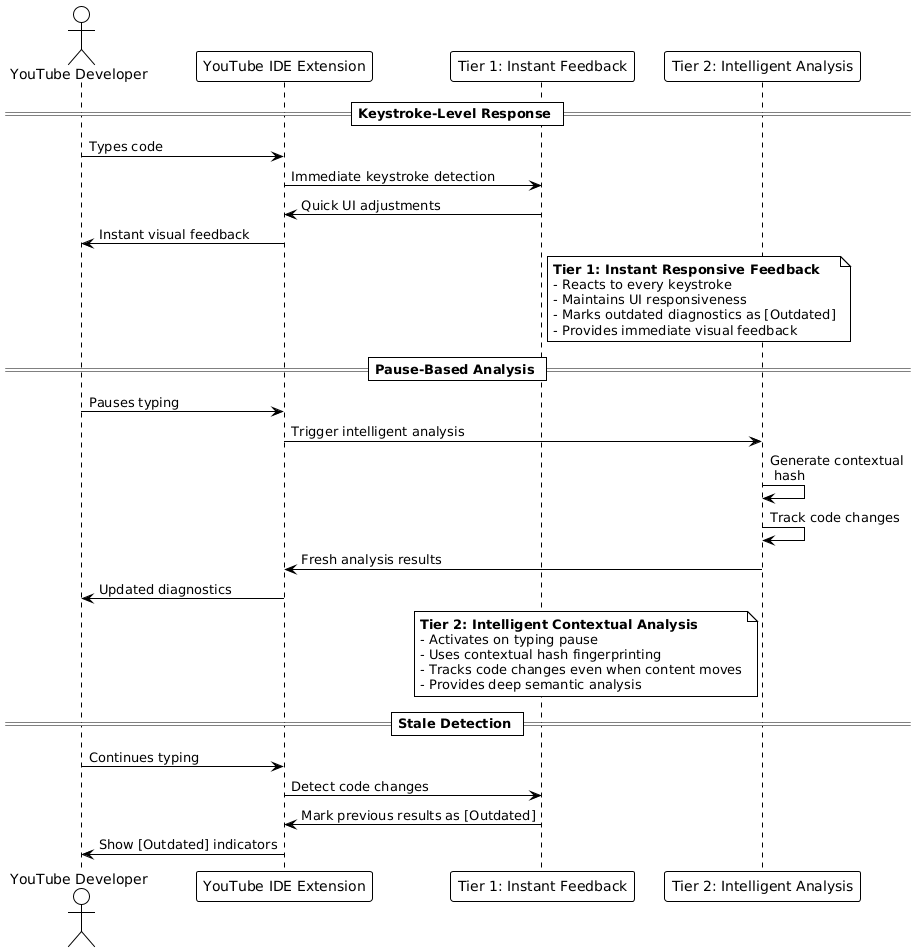
\includegraphics[scale=0.6]{images/stale_diagnostics.png}
\caption{Two-Tiered Feedback System for Handling Stale Diagnostics: Balancing instant responsiveness with intelligent analysis}
\label{fig:two_tiered_feedback}
\end{figure}

\paragraph{Tier 1: Instant Responsive Feedback}
The first tier provides immediate reaction to every keystroke, maintaining UI responsiveness through quick adjustments and intelligent state management. This tier ensures that the interface remains responsive and provides immediate visual feedback, even during rapid code changes. When analysis results become outdated due to code modifications, they are marked as [Outdated] to provide clear indication of their current relevance.

\paragraph{Tier 2: Intelligent Contextual Analysis}
The second tier activates once the developer pauses typing, employing a debounced contextual hash system, creating a unique fingerprint of the code state. This debounced approach ensures that diagnostics are re-anchored correctly after a sufficient pause in typing, maintaining responsiveness while ensuring accurate positioning. The fingerprint allows the system to track code changes even when content moves within the file, ensuring that analysis results remain relevant and accurate. The intelligent analysis tier provides deep, semantic understanding of the code while maintaining system responsiveness.

\paragraph{Seamless Integration}
The dual-tier system creates a seamless experience that balances speed with intelligence, providing developers with both immediate feedback and comprehensive analysis. This architecture represents a solution to the classic engineering problem of providing instant feedback without compromising on the depth and accuracy of AI-powered analysis.

\subsubsection{User Interaction Flow}
The complete user interaction flow with the YouTube IDE Extension is illustrated in the following diagram, showing the journey from analysis initiation to fix application:

\begin{figure}[H]
\centering
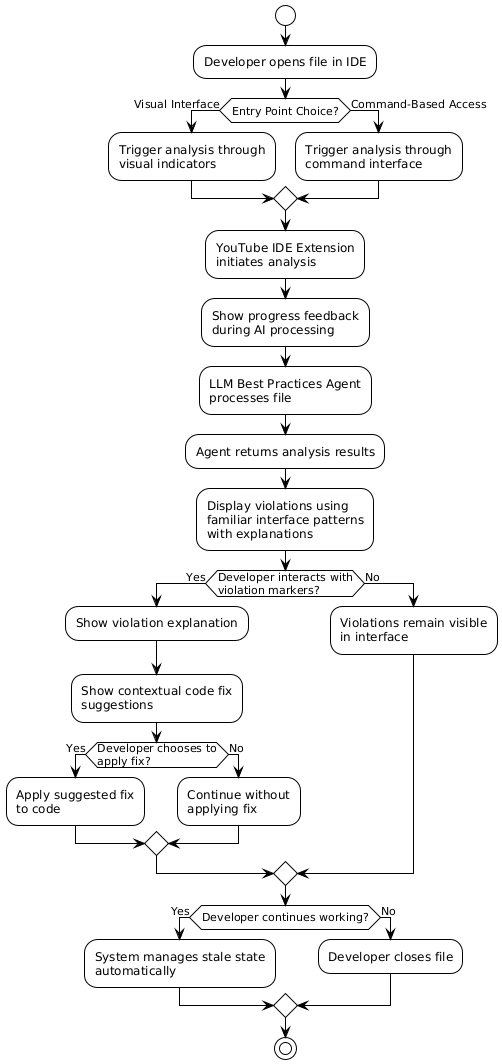
\includegraphics[scale=0.65]{images/user_flow.png}
\caption{YouTube IDE Extension User Interaction Flow: Complete developer journey from analysis trigger to fix application}
\label{fig:user_interface_flow}
\end{figure}

The flow demonstrates the key interaction patterns and decision points that YouTube developers encounter when using the extension. The process begins with analysis initiation through either the editor action or command palette, followed by real-time progress indication during AI processing. Once results are returned, violations are displayed as native IDE diagnostics with explanations. When developers hover over diagnostic markers, they receive both the explanation and formatted code fixes. The fix application process is entirely optional, allowing developers to either copy suggested changes or use the Quick Fix mechanism that calls the IDE's coding assistant. This design ensures that the AI assistance integrates naturally into existing development workflows without requiring any learning curve.


\section{Data Models and Interfaces}

\subsection{Input/Output Specification}
The system's data models define the contracts between components, ensuring consistent communication and data exchange throughout the analysis pipeline.

\paragraph{Analysis Request Format}
The YouTube IDE Extension sends analysis requests to the LLM Best Practices Agent using a simple file path string:

\begin{itemize}
    \item \textbf{File Path}: String containing the complete path to the file being analyzed. The file path must follow a specific format that includes the workspace ID and username for proper identification and access control.
\end{itemize}

This minimal input format ensures that the agent can focus on its core responsibility of code analysis while maintaining security and proper workspace isolation.

\paragraph{Analysis Response Format}
The agent returns a structured JSON response with the following top-level fields:

\begin{itemize}
    \item \textbf{status}: The overall status of the analysis: "success" or "error"
    \item \textbf{errorDetails}: Details about the error if status is "error", otherwise null
    \item \textbf{violationResults}: An array of violation objects, where each object represents a single violation found in the code
    \item \textbf{tokenUsage}: Optional object containing input\_tokens and output\_tokens if requested
\end{itemize}


Each violation object includes:

\begin{itemize}
    \item \textbf{originalViolation}: Contains the data from the initial CodeAnalysisTool pass
    \begin{itemize}
        \item \textbf{conventionId}: The unique identifier for the best practice that was violated (e.g., "local-components-complexity")
        \item \textbf{range}: The location of the violation in the source file with precise line and character positions (start/end)
    \end{itemize}
    \item \textbf{explanation}: The human-readable explanation of the violation, generated by the ViolationExplanationTool
    \item \textbf{suggestedFix}: A human-readable fix presented in the IDE hover, designed for clear rendering (formatted code snippets, e.g., TypeScript, or concise step-by-step instructions)
\end{itemize}

A minimal example response:
\begin{verbatim}
{
  "status": "success",
  "violationResults": [
    {
      "originalViolation": {
        "conventionId": "local-components-complexity",
        "range": {"start": {"line": 15, "character": 0}, 
                  "end": {"line": 15, "character": 20}}
      },
      "explanation": "This component exceeds the 
	  recommended complexity threshold.",
      "suggestedFix": "Consider breaking this into smaller components."
    }
  ],
  "tokenUsage": {"input_tokens": 150, "output_tokens": 45}
}
\end{verbatim}

\subsection{Convention Data Management}
YouTube framework best practices are stored as JSON files in the repository and imported by the agent at runtime. This approach provides version control integration and enables easy maintenance of convention definitions.

\paragraph{Rationale for JSON-Based Convention Storage}
The system stores YouTube framework best practices as JSON files rather than using a traditional database for several reasons:
\begin{itemize}
    \item \textbf{Read-Only Nature}: Conventions are static during runtime, requiring no dynamic updates, making a simple file sufficient.
    \item \textbf{Version Control}: Storing conventions in the repository allows easy tracking of changes, rollbacks, and collaboration with minimal infrastructure.
    \item \textbf{Simplicity \& Portability}: JSON files are lightweight, easy to parse, and can be loaded efficiently at agent startup without introducing database dependencies.
    \item \textbf{Performance Consideration}: Loading all conventions into memory ensures low-latency access for the AI agent during code analysis.
    \item \textbf{Prototype Context}: This design targets a single framework for prototype development, allowing quick iteration. The architecture remains flexible—if multi-framework support or dynamic updates are required in the future, the JSON layer can be replaced with a database or service with minimal impact on other components.
\end{itemize}
This approach balances maintainability, simplicity, and performance while demonstrating awareness of potential scalability needs.

\paragraph{Convention Data Structure}
The convention data is organized in a hierarchical format that supports both human readability and programmatic access:

\begin{itemize}
    \item \textbf{Convention Definitions}: Each convention includes:
    \begin{itemize}
        \item \textbf{Unique ID}: Identifier for programmatic reference
        \item \textbf{Category}: Grouping (e.g., "Component Structure", "Import Patterns", "Naming Conventions")
        \item \textbf{Description}: Clear explanation of the best practice
        \item \textbf{Examples}: Code snippets showing correct and incorrect implementations
        \item \textbf{Rationale}: Explanation of why this practice improves code quality
        \item \textbf{Severity}: Default severity level for violations
    \end{itemize}
    \item \textbf{Dynamic Retrieval}: Context-specific data inclusion in prompts based on:
    \begin{itemize}
        \item File type and framework context
        \item Previously detected violations in the same file
    \end{itemize} 
\end{itemize} 

\paragraph{Integration Interfaces}
The following minimal, versioned boundaries keep components decoupled. Detailed request/response fields are defined earlier in Input/Output Specification.

\begin{itemize}
    \item \textbf{IDE Extension Interface}: AnalysisRequest/AnalysisResponse contract between the YouTube IDE Extension and the LLM Best Practices Agent. Requests include the file path (workspace + username); responses follow the Analysis Response Format. This boundary lets the UI evolve independently from the agent.
    \item \textbf{Convention Access}: The agent loads a local JSON array of convention definitions at startup (read-only). This simple import avoids network dependencies and provides direct access to IDs, descriptions, examples, and severity.
    \item \textbf{Monitoring Interface}: Captures token usage from LLM method calls and aggregate counts of violations by category for observability. Latency and accuracy measurements are discussed in the Evaluation chapter.
\end{itemize}


\subsection*{Conclusion}
The architecture of the LLM Best Practices Agent is defined by three central design decisions. First, the adoption of the Executable Agent paradigm ensures deterministic execution, structured tool orchestration, and predictable performance, avoiding the drawbacks of open-ended reasoning loops. Second, the hybrid parallel–sequential processing strategy balances efficiency with interpretability, allowing analyses to scale while maintaining transparency in intermediate results. Finally, the IDE extension provides a seamless developer experience, integrating diagnostics, explanations, and fixes directly into familiar workflows while managing state and staleness automatically. Together, these pillars create a robust, cost-efficient, and developer-friendly system for embedding AI-driven best practice enforcement into the coding environment.
%==============================================================================
\end{spacing}
